\begin{figure}[htbp]
    \centering
    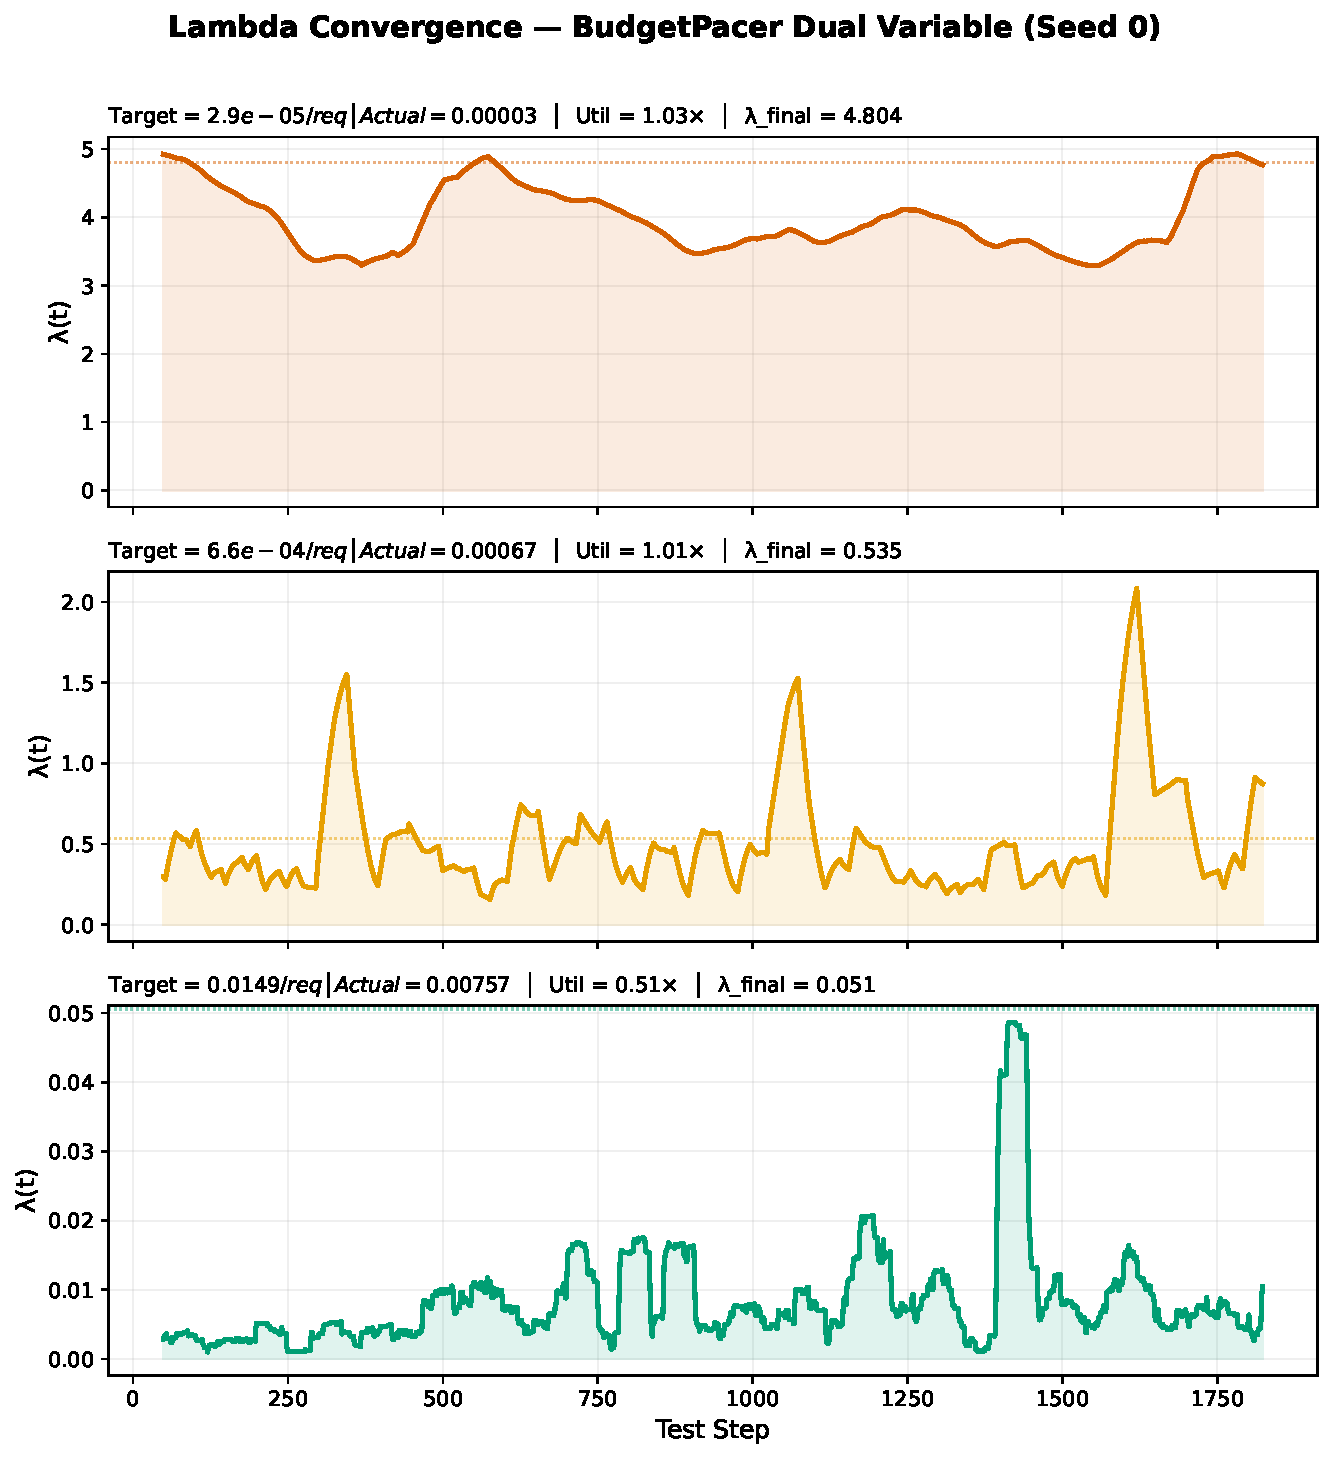
\includegraphics[width=\linewidth]{../experiments_v2/01_stationary_budget_pacing/results/lambda_convergence.pdf}
    \caption{Dual-variable trajectory $\lambda_t$ over the 1{,}824-step
    test phase (seed~0) at three representative budget targets.
    %
    \textbf{Top} (tight, $B{=}\$2.9{\times}10^{-5}$/req):
    $\lambda_t$ saturates near the cap $\bar\lambda{=}5$, forcing
    near-exclusive Llama routing (99.9\%).  The hard ceiling filters
    Mistral and Gemini outright; the soft penalty is redundant.
    Budget utilisation: $1.03\times$.
    %
    \textbf{Middle} (moderate, $B{=}\$6.6{\times}10^{-4}$/req):
    $\lambda_t$ oscillates around $0.3$--$0.5$, actively balancing a
    Llama/Mistral mix (51\%/46\%).  Spikes correspond to occasional
    Gemini selections ($2.6\%$) whose high cost drives a transient
    overspend; the dual variable corrects within ${\sim}20$ steps.
    Budget utilisation: $1.01\times$.
    %
    \textbf{Bottom} (loose, $B{=}\$0.015$/req):
    The target exceeds the unconstrained router's natural spend;
    $\lambda_t$ hovers near zero, exerting negligible influence.
    The selection mix (9\% Llama, 44\% Mistral, 47\% Gemini) matches
    the quality-optimal unconstrained policy.
    Budget utilisation: $0.51\times$ (the router cannot be \emph{forced}
    to spend more).
    %
    The 50-step moving average (solid line) shows the smoothed trend;
    the dotted horizontal line marks $\lambda_{\text{final}}$.
    Across all targets, $\lambda_t$ stabilises within the first
    ${\sim}300$ test steps, demonstrating rapid convergence of the
    primal-dual scheme.
    }
    \label{fig:lambda_convergence}
\end{figure}
